\documentclass[aspectratio=169, 10pt]{beamer}

\usepackage[utf8]{inputenc}
\usepackage[english]{babel}
\usepackage[T1]{fontenc}
\usepackage{csquotes}
\usepackage{lmodern}
\usepackage{hyperref}
\usepackage{url}
\usepackage{graphicx}
\usepackage{marvosym}

\setbeamertemplate{navigation symbols}{}
\usetheme{TUBlayout}
\pdfstringdefDisableCommands{%
  \def\includegraphics{}%
  \def\textwidth{}%
}
\newcommand{\arrow}{\Large \MVRightarrow}

\title[Ecovisor \& Mosaik Co-Simulation]{
    
\includegraphics[width=.4\textwidth]{mosaik}\\[7mm]
    Integrating Ecovisor into Mosaik Co-Simulation\\
    \normalsize Simulate the Virtual Energy Grid
}
\author[Nickel \& Steinke]{Henrik Nickel, Marvin Steinke}
\institute{Technische Universität Berlin}
\newcommand{\preslocation}{Berlin}
\date{\today}

\begin{document}

\frame[plain]{\titlepage}

\section{Previous Design}
%\frame[noframenumbering]{\sectionpage}
\begin{frame}
    \begin{columns}[c]
        \column{.5\textwidth}
        \begin{figure}
            \centering
            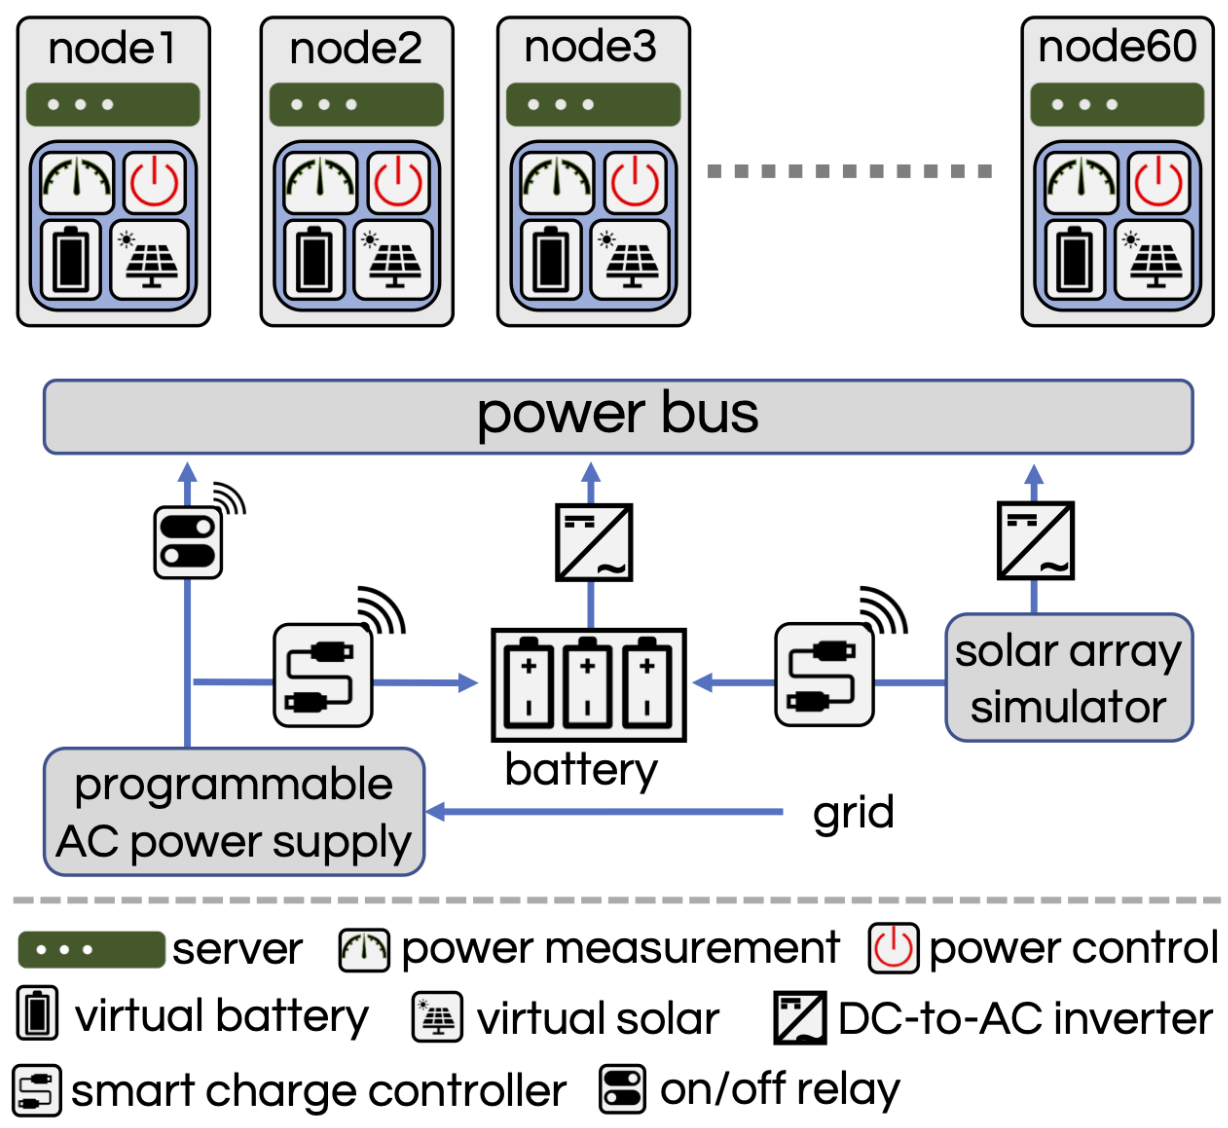
\includegraphics[width=.7\textwidth]{ecovisor_energy_system}
            \caption{Ecovisor energy system, adapted from Souza et al. [1]}
            \label{fig:ecovisor_energy_system}
        \end{figure}
        \column{.5\textwidth}
        \begin{figure}
            \centering
            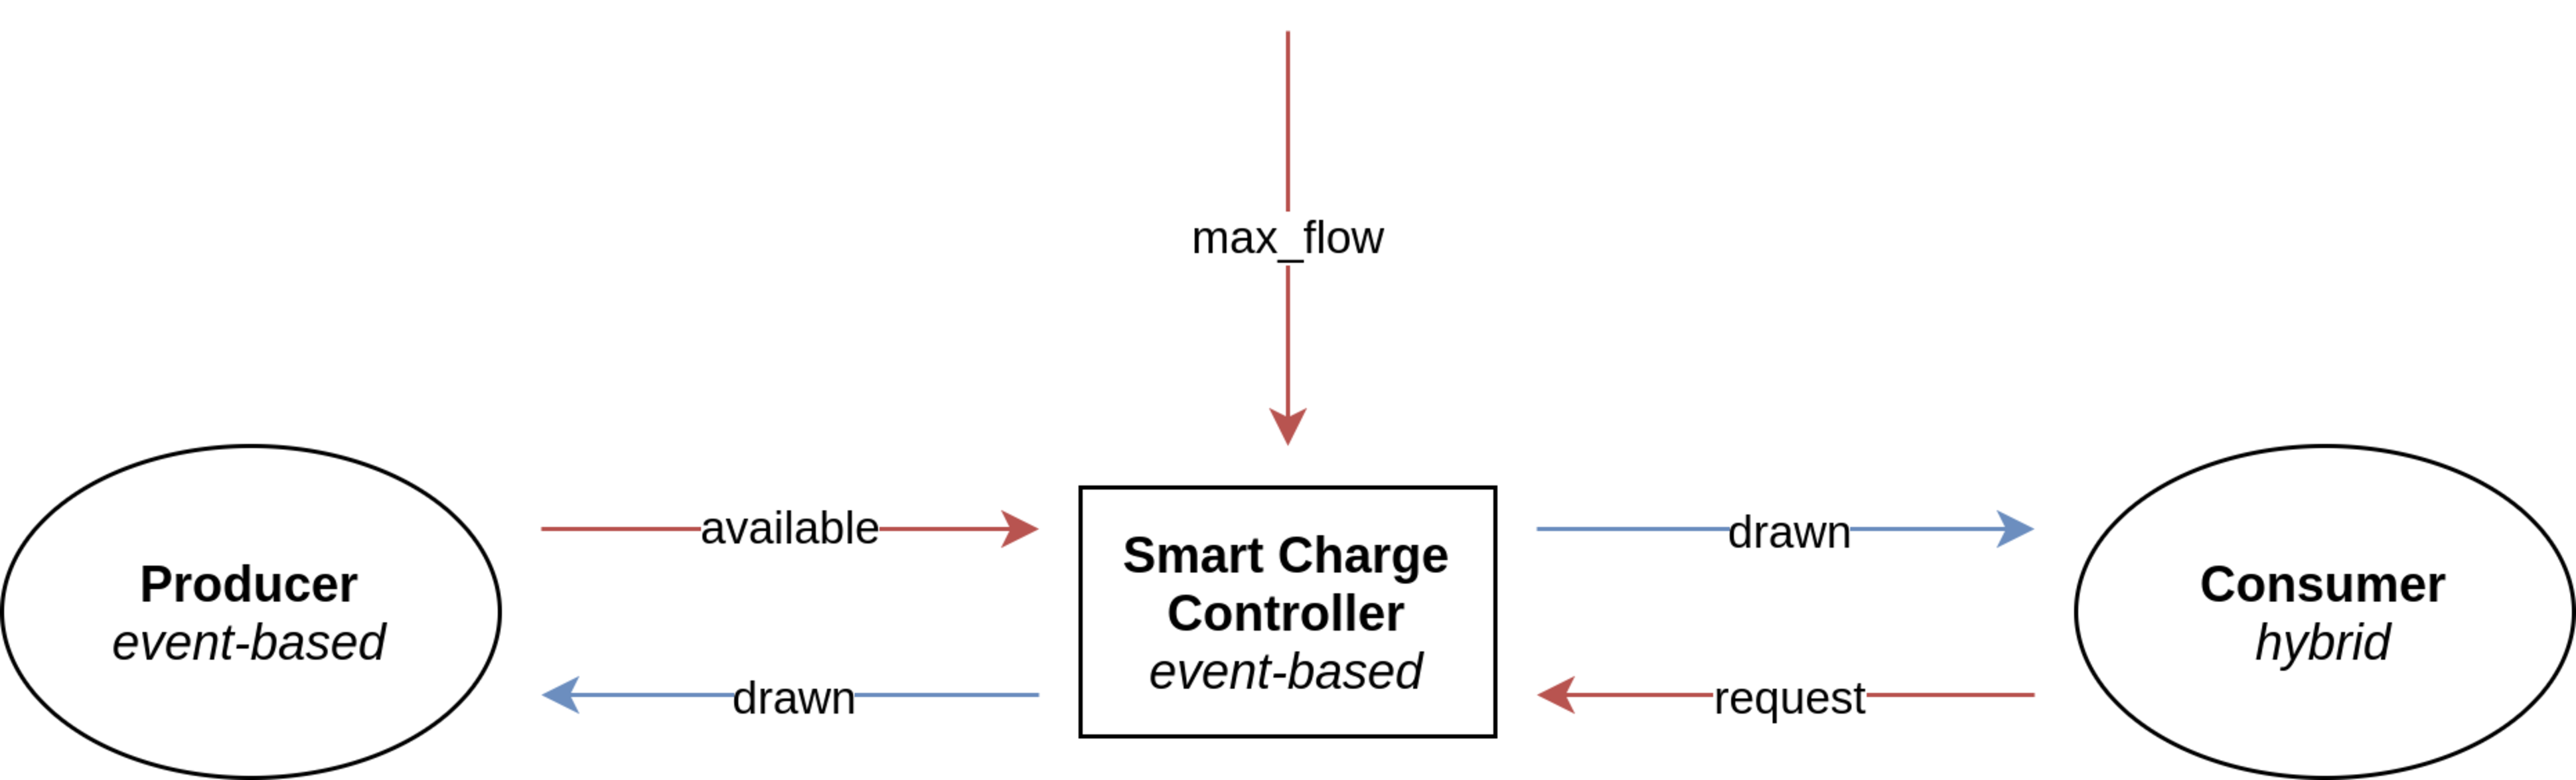
\includegraphics[width=\textwidth]{../smart_charge_controller.pdf}
            \caption{Smart-charge-controller}
            \label{fig:smart_charge_controller}
        \end{figure}
    \end{columns}
\end{frame}

\section{Current Design}
%\frame[noframenumbering]{\sectionpage}
\begin{frame}
    \begin{columns}[c]
        \column{.5\textwidth}
        \begin{figure}
            \centering
            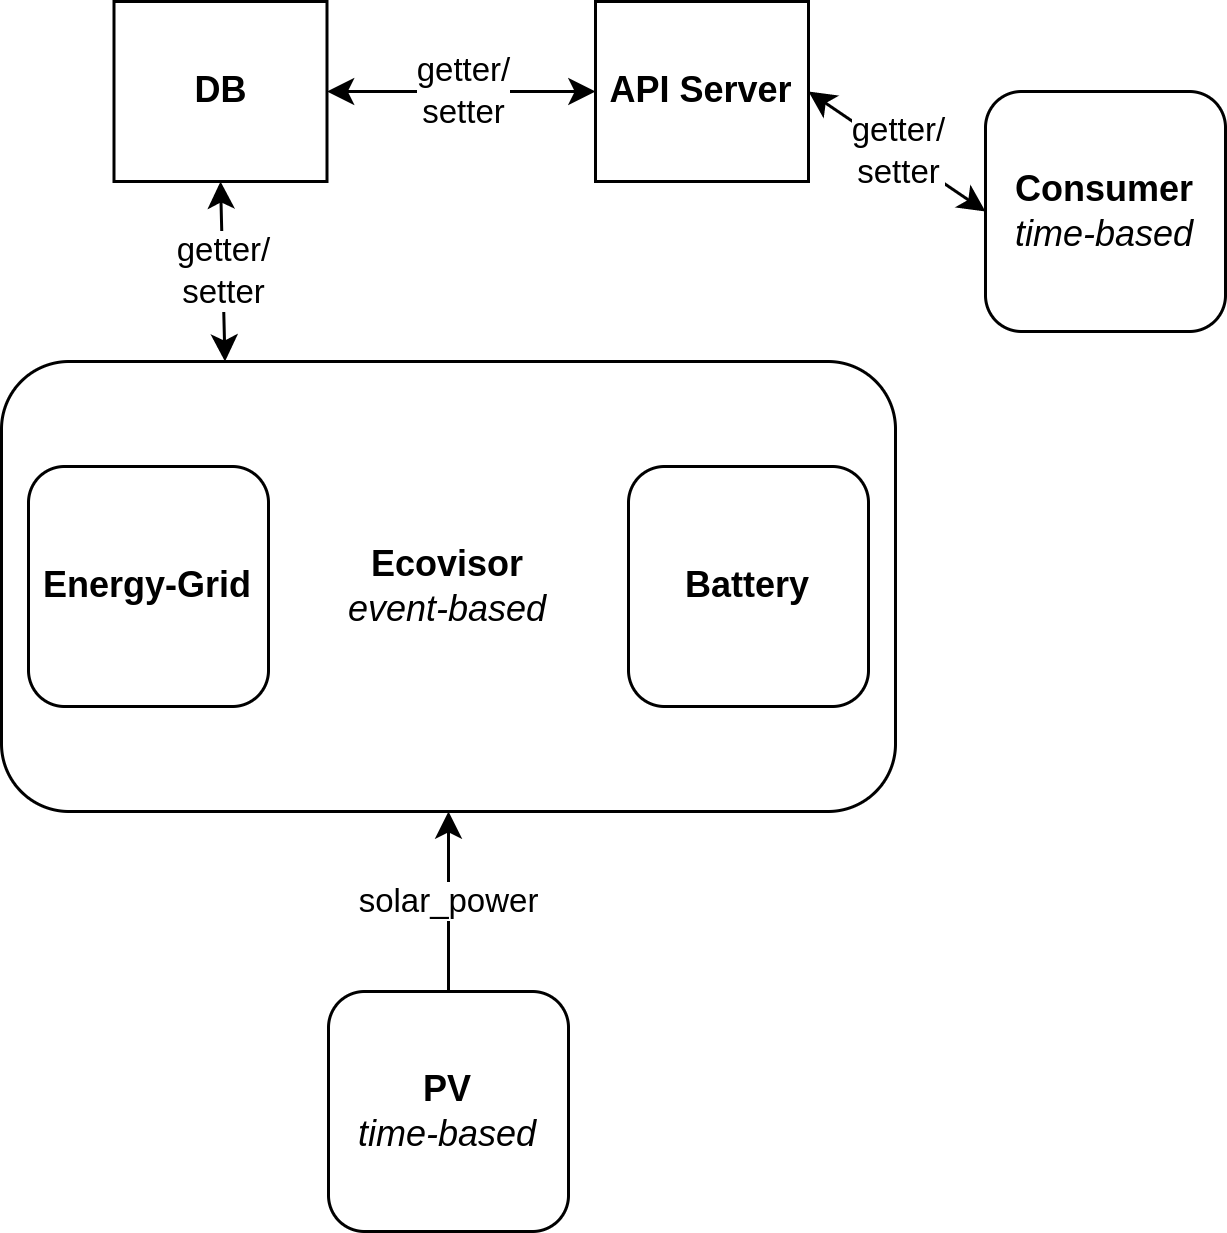
\includegraphics[height=5cm]{../sketch.png}
            \caption{Ecovisor design integration}
            \label{fig:ecovisor_testbed}
        \end{figure}
        \column{.5\textwidth}
        \begin{itemize}
            \item battery and energy-grid interface directly integrated into Ecovisor
            \vspace{3mm}
            \item DB + API Server allows for multiple client connections
            \vspace{3mm}
            \item Remaining: Consumer
        \end{itemize}
    \end{columns}
\end{frame}

\appendix

\begin{frame}[noframenumbering]{%
        Questions?\\
        \normalsize And thank you for your attention
}
\begin{itemize}
    \item[{[1]}] A. Souza, N. Bashir, J. Murillo, W. Hanafy, Q. Liang, D. Irwin, and P.
        Shenoy, “Ecovisor: A virtual energy system for carbon-efficient
        applications,” arXiv preprint arXiv:2210.04951, 2022.
\end{itemize}
\vspace{4mm}
\begin{itemize}
    \item title page graphics adapted from \url{https://mosaik.offis.de/}
\end{itemize}
\end{frame}

\end{document}
